In Aufgaben~\ref{40000078} wurde erkannt, dass die dortige Grammatik
nicht eindeutig ist und die zwei Parse Trees
\begin{center}
\raisebox{-2.0cm}{
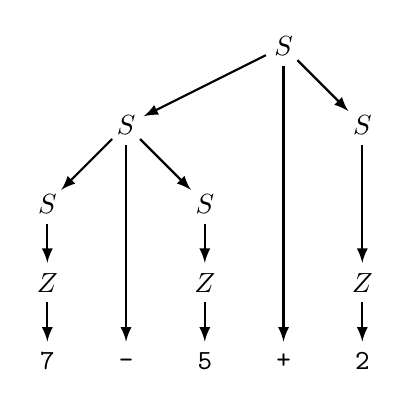
\begin{tikzpicture}[>=latex,thick]
\coordinate (S1) at (3,4);
\coordinate (S2) at (4,3);
\coordinate (S3) at (1,3);
\coordinate (S4) at (0,2);
\coordinate (S5) at (2,2);
\coordinate (Z1) at (0,1);
\coordinate (Z2) at (2,1);
\coordinate (Z3) at (4,1);
\coordinate (T1) at (0,0);
\coordinate (T2) at (1,0);
\coordinate (T3) at (2,0);
\coordinate (T4) at (3,0);
\coordinate (T5) at (4,0);
\node at (S1) {$S$};
\draw[->,shorten >= 0.25cm,shorten <= 0.25cm] (S1) -- (S2);
\draw[->,shorten >= 0.25cm,shorten <= 0.25cm] (S1) -- (S3);
\draw[->,shorten >= 0.25cm,shorten <= 0.25cm] (S1) -- (T4);
\node at (S2) {$S$};
\draw[->,shorten >= 0.25cm,shorten <= 0.25cm] (S2) -- (Z3);
\node at (S3) {$S$};
\draw[->,shorten >= 0.25cm,shorten <= 0.25cm] (S3) -- (S4);
\draw[->,shorten >= 0.25cm,shorten <= 0.25cm] (S3) -- (T2);
\draw[->,shorten >= 0.25cm,shorten <= 0.25cm] (S3) -- (S5);
\node at (S4) {$S$};
\draw[->,shorten >= 0.25cm,shorten <= 0.25cm] (S4) -- (Z1);
\node at (S5) {$S$};
\draw[->,shorten >= 0.25cm,shorten <= 0.25cm] (S5) -- (Z2);
\node at (Z1) {$Z$};
\node at (Z2) {$Z$};
\node at (Z3) {$Z$};
\draw[->,shorten >= 0.25cm,shorten <= 0.25cm] (Z1) -- (T1);
\draw[->,shorten >= 0.25cm,shorten <= 0.25cm] (Z2) -- (T3);
\draw[->,shorten >= 0.25cm,shorten <= 0.25cm] (Z3) -- (T5);
\node at (T1) {\texttt{7}};
\node at (T2) {\texttt{-}};
\node at (T3) {\texttt{5}};
\node at (T4) {\texttt{+}};
\node at (T5) {\texttt{2}};
\end{tikzpicture}}
\qquad\text{und}\qquad
\raisebox{-2.0cm}{
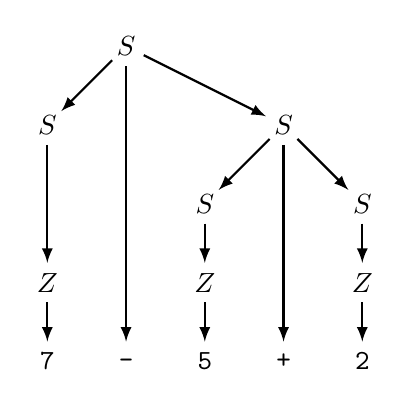
\begin{tikzpicture}[>=latex,thick]
\coordinate (S1) at (1,4);
\coordinate (S2) at (0,3);
\coordinate (S3) at (3,3);
\coordinate (S4) at (2,2);
\coordinate (S5) at (4,2);
\coordinate (Z1) at (0,1);
\coordinate (Z2) at (2,1);
\coordinate (Z3) at (4,1);
\coordinate (T1) at (0,0);
\coordinate (T2) at (1,0);
\coordinate (T3) at (2,0);
\coordinate (T4) at (3,0);
\coordinate (T5) at (4,0);
\node at (S1) {$S$};
\draw[->,shorten >= 0.25cm,shorten <= 0.25cm] (S1) -- (S2);
\draw[->,shorten >= 0.25cm,shorten <= 0.25cm] (S1) -- (S3);
\draw[->,shorten >= 0.25cm,shorten <= 0.25cm] (S1) -- (T2);
\node at (S2) {$S$};
\draw[->,shorten >= 0.25cm,shorten <= 0.25cm] (S2) -- (Z1);
\node at (S3) {$S$};
\draw[->,shorten >= 0.25cm,shorten <= 0.25cm] (S3) -- (S4);
\draw[->,shorten >= 0.25cm,shorten <= 0.25cm] (S3) -- (T4);
\draw[->,shorten >= 0.25cm,shorten <= 0.25cm] (S3) -- (S5);
\node at (S4) {$S$};
\draw[->,shorten >= 0.25cm,shorten <= 0.25cm] (S4) -- (Z2);
\node at (S5) {$S$};
\draw[->,shorten >= 0.25cm,shorten <= 0.25cm] (S5) -- (Z3);
\node at (Z1) {$Z$};
\node at (Z2) {$Z$};
\node at (Z3) {$Z$};
\draw[->,shorten >= 0.25cm,shorten <= 0.25cm] (Z1) -- (T1);
\draw[->,shorten >= 0.25cm,shorten <= 0.25cm] (Z2) -- (T3);
\draw[->,shorten >= 0.25cm,shorten <= 0.25cm] (Z3) -- (T5);
\node at (T1) {\texttt{7}};
\node at (T2) {\texttt{-}};
\node at (T3) {\texttt{5}};
\node at (T4) {\texttt{+}};
\node at (T5) {\texttt{2}};
\end{tikzpicture}}

\end{center}
für den Ausdruck \texttt{7-5+2} zulässt.
Formulieren Sie Regeln für die Auswertung des Parse Tree und bestimmen
Sie die Werte des Ausdrucks für die beiden Parse Trees.

\begin{loesung}
Die Auswerteregel lautet:
Der Wert eines $S$-Knotes des Parse-Trees ist entweder die daraus
abgeleitet Zahl $Z$, oder die Summe bzw.~Different der Werte der beiden
darunter liegenden $S$-Knoten, je nach der Operation in der Mitte.
Die beiden Parse-Trees haben nach diesen Regeln die Werte
\begin{align*}
\text{links:\qquad}&(7-5)+2=4
&
\text{rechts:\qquad}&7-(5+2)=0
\end{align*}
Der Wert des rechten Parse-Trees ist offensichtlich falsch.
Diese Grammatik ist ungeeignet, um die korrekte Auswertung
von Ausdrücken sicherzustellen.
\end{loesung}


